\chapter{呼吸}\label{ch:g4:breathing}

屏住\omterm{def:g4:breathing:movements}{呼吸}，开始数数。远在一分钟之前，
胸部便越来越迫切地要求再次\omterm{def:g4:breathing:movements}{呼吸}。你
可以少吃一顿饭，\omterm{prop:g1:healthy-habits:needs}{睡眠}可以等到今晚——而空气
却需要\emph{立即}补充，日夜不停，每分钟约十五次。
一口空气，为何如此紧迫？

\section{呼吸的两个动作}

\begin{definition}[吸气与呼气]\label{def:g4:breathing:movements}
\emph{呼吸}\index{呼吸}是
两种动作的不断交替：
\begin{itemize}
  \item \emph{吸气}\,\index{吸气}：
        胸腔扩张，空气经鼻或口进入；
  \item \emph{呼气}\,\index{呼气}：
        胸腔回缩，空气被排出。
\end{itemize}
安静时，一吸一呼约每分钟重复 $15$ 次——
婴儿更快，用力时也更快，你
无需刻意去想。
\end{definition}

\begin{example}[观察呼吸动作]\label{ex:g4:breathing:watch}
双手平放在\omterm{def:g3:bones-and-muscles:skeleton}{肋骨}上：\omterm{def:g4:breathing:movements}{吸气}时，胸廓抬起并
在掌下扩张；\omterm{def:g4:breathing:movements}{呼气}时，胸廓回落。
熟睡的猫的侧腹也呈现同样的起伏。这
些动作从不停止——醒着、睡着，从第一声啼哭
到最后一天。
\end{example}

\section{空气去往何处}

\begin{definition}[呼吸器官]\label{def:g4:breathing:organs}
吸入的空气经由鼻（或口），
向下进入\emph{气管}\index{气管}——一根结实的环状管子，你
颈部前方即可摸到，它分为两
支，分别通向每一侧的\emph{肺}\index{肺}。两个肺，
是充满胸腔的海绵状器官，
（位于\omterm{def:g3:bones-and-muscles:skeleton}{肋骨}之后，见\cref{def:g3:bones-and-muscles:skeleton}），
末端是数以百万计的微小气囊，
每个气囊外包细小血管。
\end{definition}

\begin{omfigure}
\begin{tikzpicture}
  \node[anchor=south west, inner sep=0] (img) at (0,0)
    {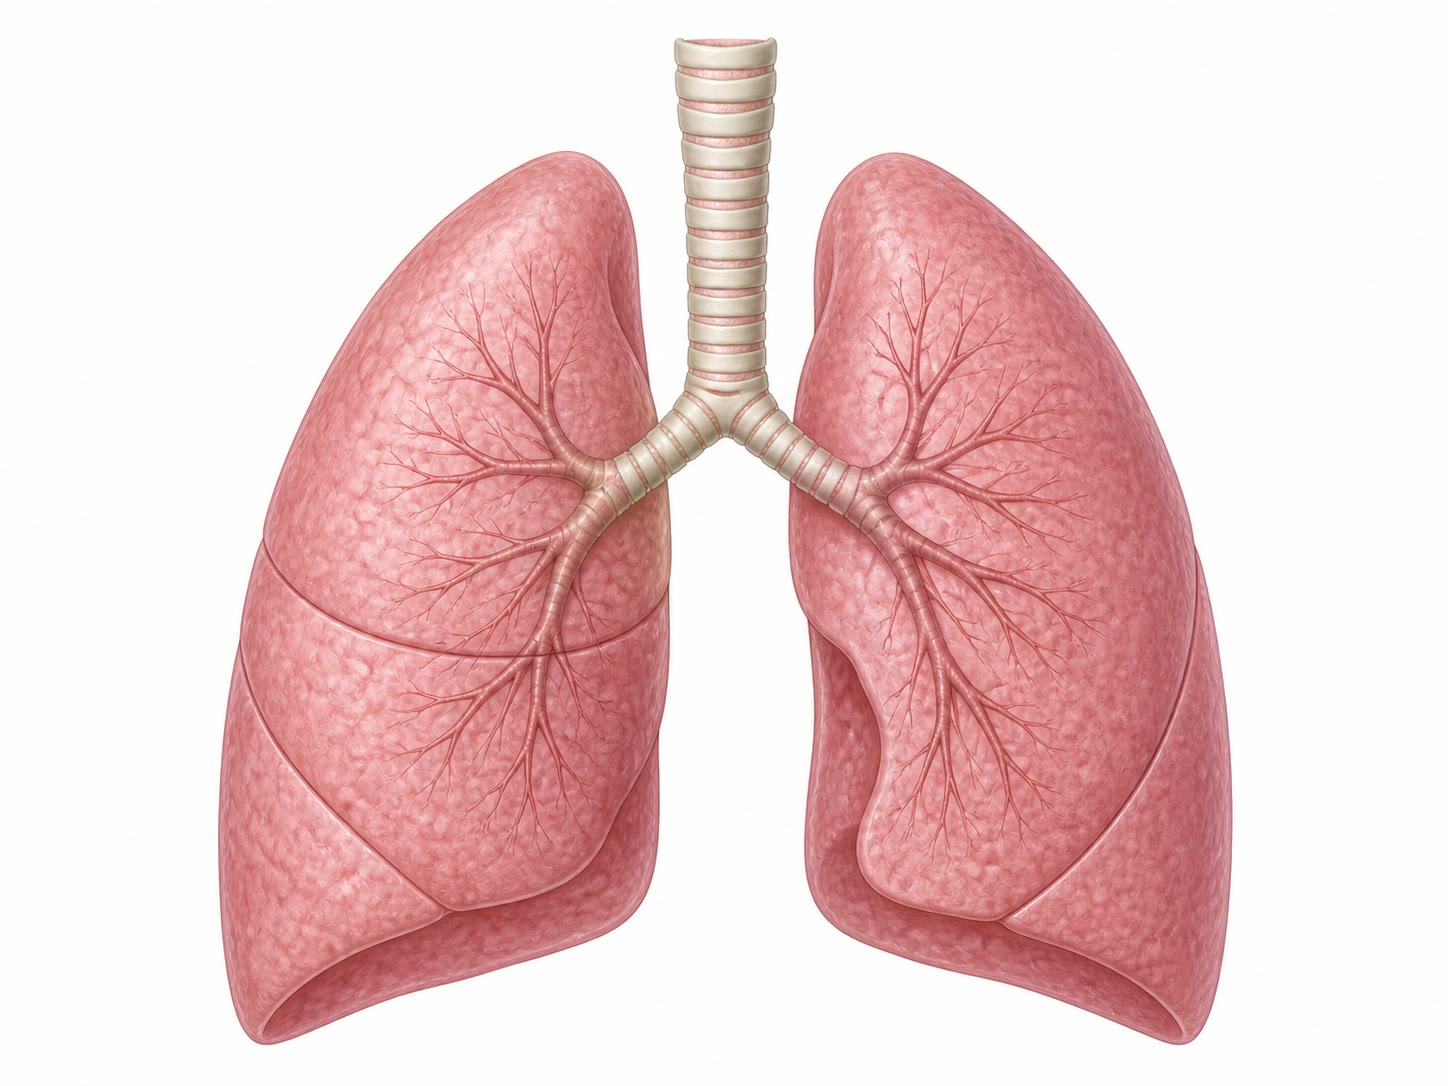
\includegraphics[width=0.58\linewidth]{images/book1/ai/fig-lungs.jpg}};
  \begin{scope}[x={(img.south east)}, y={(img.north west)},
      every node/.style={font=\small}]
    \draw[omDef, thick] (0.53,0.88) -- (0.74,0.93) node[right] {气管};
    \draw[omDef, thick] (0.585,0.61) -- (1.03,0.64)
      node[right, align=left] {两个 \\ 分支};
    \draw[omDef, thick] (0.28,0.28) -- (0.11,0.13)
      node[below] {肺};
  \end{scope}
\end{tikzpicture}

{\small 一次\omterm{def:g4:breathing:movements}{呼吸}的路径：\omterm{def:g4:breathing:organs}{气管}、两个\omterm{def:g1:plants-around-us:tree}{分支}、两个肺
——以及在\omterm{def:g1:plants-around-us:tree}{分支}最细的末端，有数以百万计的微小气囊，
外包细小血管，远小到
本图比例下无法看清。}
\end{omfigure}

\begin{remark}[海绵状结构的妙处]\label{rem:g4:breathing:sponge}
数百万个气囊，而非两个简单的囊袋：这
又是\omterm{def:g4:journey-of-food:tract}{小肠}的同一妙招
（见\cref{rem:g4:journey-of-food:surface}）。所有这些囊壁
相加，形成空气与
\omterm{prop:g4:journey-of-food:absorb}{血液}之间巨大的接触面——约半个网球场大小，折叠在
你的胸腔内。
\end{remark}

\section{呼吸的作用}

\begin{proposition}[吸入氧气，排出二氧化碳]\label{prop:g4:breathing:exchange}
空气是多种气体的混合物，人体需要其中的一种：
\emph{氧气}\index{氧气}。在肺的气囊中，氧气
从新鲜空气中进入\omterm{prop:g4:journey-of-food:absorb}{血液}，\omterm{prop:g4:journey-of-food:absorb}{血液}将其输送至
身体的每个部位；在那里，它与\omterm{def:g4:journey-of-food:digestion}{营养物质}
一起被利用，以释放\omterm{prop:g3:balanced-diet:jobs}{能量}（
见\cref{prop:g3:balanced-diet:jobs}）。人体的废气，
\emph{二氧化碳}\index{二氧化碳}则走上返程，
被呼出。呼出的空气中氧气较少、
二氧化碳较多，与吸入的空气相比——
这一差别正是\omterm{def:g4:breathing:movements}{呼吸}的\emph{意义}。
\end{proposition}
\admitted

\begin{example}[为何跑步会让人喘不过气]\label{ex:g4:breathing:running}
短跑时，双腿快速消耗\omterm{prop:g3:balanced-diet:jobs}{能量}——因此需要
快速的氧气供应。\omterm{def:g4:breathing:movements}{呼吸}随之加快：由安静时每分钟约 $15$ 次
平稳\omterm{def:g4:breathing:movements}{呼吸}，增至每分钟 $40$ 次以上，且更深，同时心脏
（见\cref{ch:g4:heart-and-blood}）加速跳动，以加快
输送。比赛后的喘息，是身体
在结清其氧气“欠账”。
\end{example}

\begin{example}[起雾的镜子]\label{ex:g4:breathing:mirror}
对着冷镜子\omterm{def:g4:breathing:movements}{呼气}：镜面起雾。呼出的空气
已经改变——变暖、变湿，并且悄悄地
氧气减少、二氧化碳增多。镜子能显示的是
水汽；镜子无法显示的气体交换，才是要点。
\end{example}

\begin{omfigure}
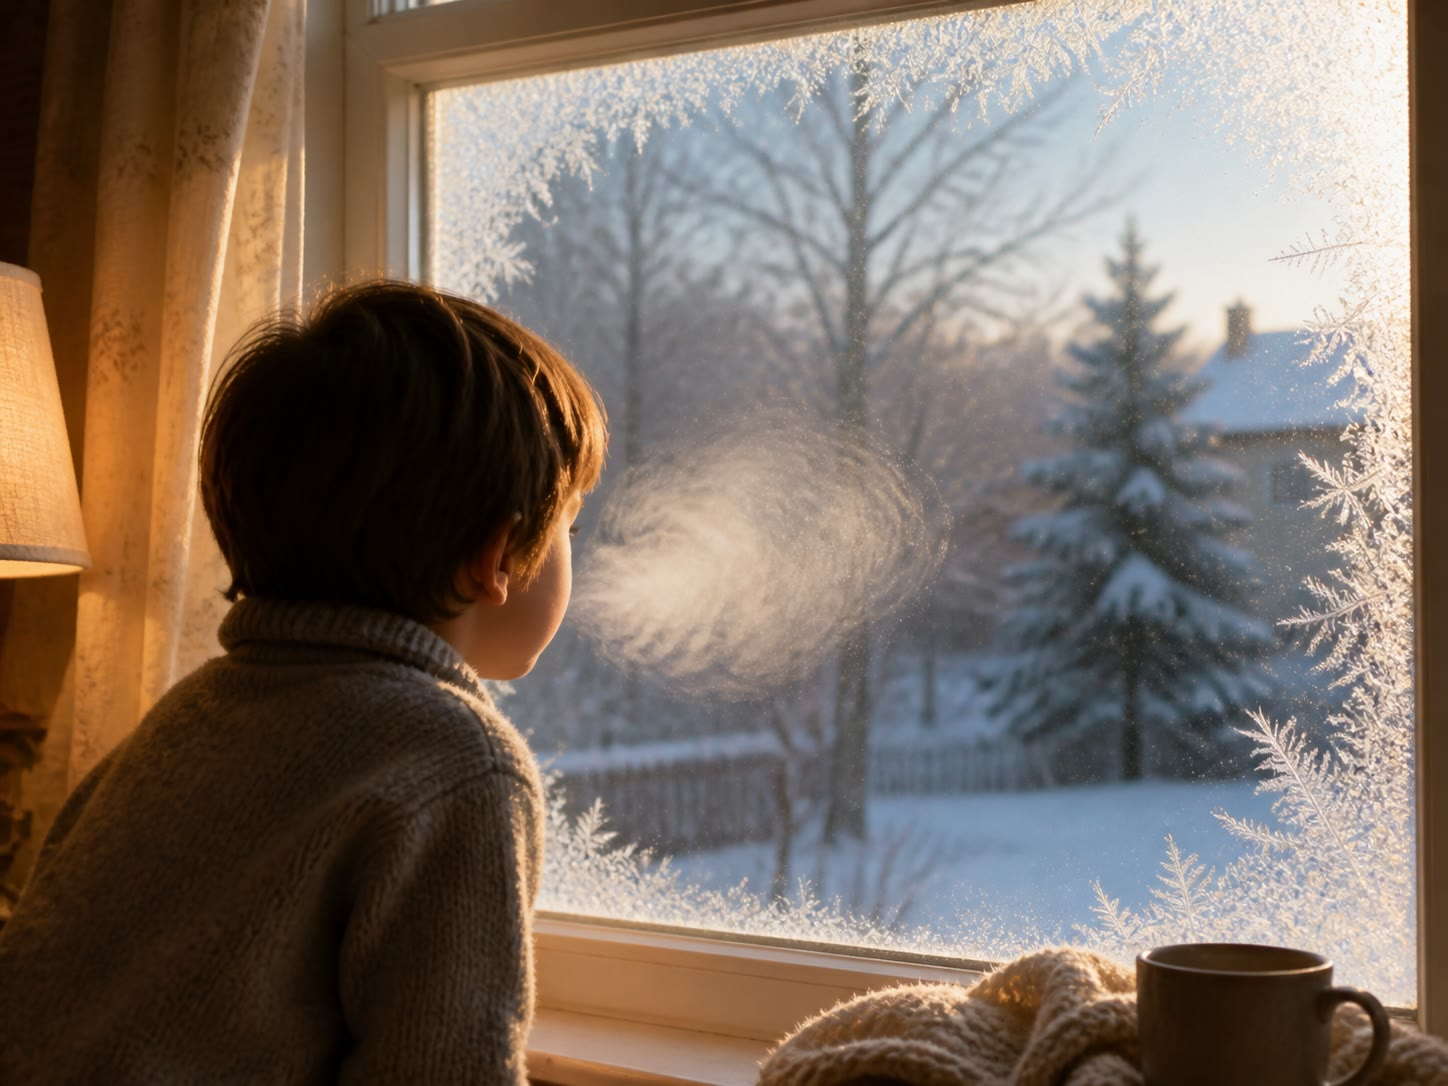
\includegraphics[width=0.56\linewidth]{images/book1/ai/g4-breathing-mist.jpg}

{\small 呼出的空气可见：温暖、潮湿——并且无形中
氧气减少，二氧化碳增多。}
\end{omfigure}

\begin{method}[呼吸的护理]\label{met:g4:breathing:care}
\begin{enumerate}
  \item 每天给房间通风——密闭房间里人多时，
        空气会变得沉闷，二氧化碳含量高；
  \item 寒冷或多尘的空气中，应用鼻子\omterm{def:g4:breathing:movements}{呼吸}：空气
        会被加温、湿润并过滤；
  \item 跑步、游泳、玩耍——经常锻炼的肺和\omterm{def:g4:breathing:movements}{呼吸}
        \omterm{def:g3:bones-and-muscles:muscle}{肌肉}会更强壮，\omterm{def:g4:breathing:movements}{呼吸}也更深；
  \item 让烟雾远离肺部：它会弄脏
        细嫩的肺泡，而肺泡只能
        缓慢地自行清洁。
\end{enumerate}
\end{method}

\section{练习}

\begin{exercise}[$\star$]\label{exo:g4:breathing:1}
说出两种\omterm{def:g4:breathing:movements}{呼吸}运动，以及胸部在
每种运动中的变化。
\end{exercise}

\begin{exercise}[$\star$]\label{exo:g4:breathing:2}
追踪一次\omterm{def:g4:breathing:movements}{呼吸}的路径：从鼻子到微小的肺泡。
\end{exercise}

\begin{exercise}[$\star$]\label{exo:g4:breathing:3}
安静休息的儿童每分钟大约
\omterm{def:g4:breathing:movements}{呼吸}多少次？冲刺时这个次数会怎样变化，
为什么？
\end{exercise}

\begin{exercise}[$\star$]\label{exo:g4:breathing:4}
身体从空气中摄取哪种气体，又放回哪种气体？
这种交换究竟发生在哪里？
\end{exercise}

\begin{exercise}[$\star$]\label{exo:g4:breathing:5}
呼出的空气与吸入的空气有何不同？请说出
三点不同。
\end{exercise}

\begin{exercise}[$\star$]\label{exo:g4:breathing:6}
为什么肺由数百万个微小的肺泡构成，
而不是两个简单的囊袋？本学年学过的哪个器官
也采用了同样的办法？
\end{exercise}

\begin{exercise}[$\star$]\label{exo:g4:breathing:7}
为什么在严寒或多尘的日子里
用鼻子\omterm{def:g4:breathing:movements}{呼吸}更好？
\end{exercise}

\begin{exercise}[$\star$]\label{exo:g4:breathing:8}
动手试一试：安静地坐着，数一分钟内的\omterm{def:g4:breathing:movements}{呼吸}次数。
然后做二十个开合跳，再数一次。记录两次的
数字，并解释其变化。
\end{exercise}

\begin{exercise}[$\star\star$]\label{exo:g4:breathing:9}
进餐可以等几个小时，\omterm{def:g4:breathing:movements}{呼吸}却不能等一分钟。这说明
身体储存氧气的量与其食物储备相比，
情况如何？
\end{exercise}

\begin{exercise}[$\star\star$]\label{exo:g4:breathing:10}
到上午晚些时候，教室的空气感觉“闷”。
由\cref{prop:g4:breathing:exchange}可知，教室空气发生了什么变化，
而\cref{met:g4:breathing:care}给出了什么做法？
\end{exercise}

\begin{exercise}[$\star\star\star$]\label{exo:g4:breathing:11}
鳟鱼没有肺：水流经过它\omterm{def:g1:animals-around-us:covering}{羽毛}状的鳃，
水中\emph{溶解于水中的}氧气就在此进入其
\omterm{prop:g4:journey-of-food:absorb}{血液}。鳃和肺有什么共同的功能？为什么
鳟鱼在氧气充足的空气中却会窒息？
（提示：离开水后，\omterm{def:g1:animals-around-us:covering}{羽毛}状的鳃表面会塌陷，
并粘在一起。）
\end{exercise}
